\section{Magnetohydrodynamics II, Geometric Optics I}

Last class, we assembled a set of equations corresponding to the ideal MHD system. One of them was the induction equation:
\begin{equation}
    \dot{\v{B}} = \nabla \times(\v{v} \times \v{B})
\end{equation}

\subsection{Conservation of Flux through Comoving Surfaces}
Let's talk about a consequence of this equation.

We can think about a surface, which evolves in time:

\begin{center}
    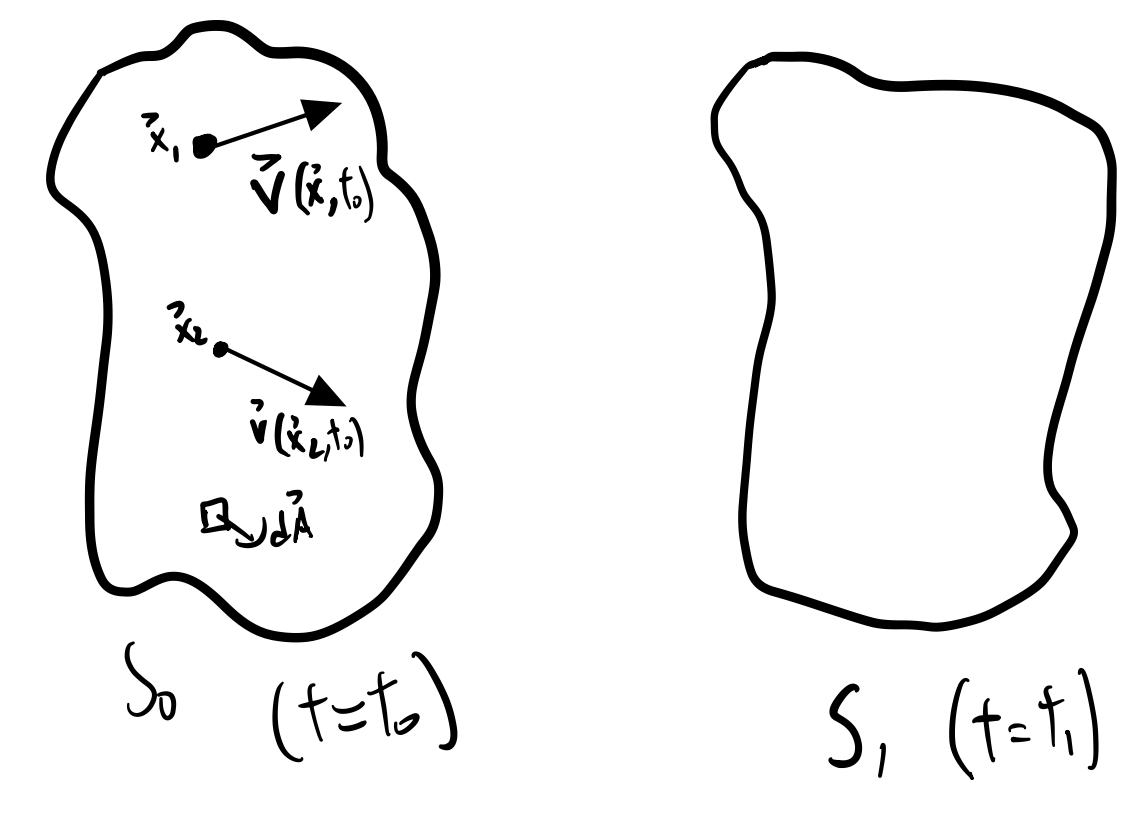
\includegraphics[scale=0.35]{Lectures/Images/lec16-twosurfaces.png}
\end{center}

The $\v{B}$-field also evolves. We can ask - what happens to the flux of the $\v{B}$-field as time goes by. The statement that we will prove next is that the flux through a comoving surface is independent of time:
\begin{equation}
    \underbrace{\int_{S_0}\v{B} \cdot d\v{A}}_{t=t_0} = \underbrace{\int_{S_1}\v{B} \cdot d\v{A}}_{t=t_1}
\end{equation}
We can imagine that the magnetic field is frozen into the fluid.

To this end, we compute:
\begin{equation}
    \dod{}{t}\int_{S(t)}\v{B} \cdot d\v{A} = 0
\end{equation}
The time derivative can hit the magnetic field $\v{B}$ as well as the surface $S(t)$:
\begin{equation}
    \dod{}{t}\int_{S(t)}\v{B} \cdot d\v{A} = \int_{S(t)} \dot{\v{B}} \cdot d\v{A} + \frac{\delta}{\delta t}\int_{S(t)}\v{B} \cdot d\v{A}
\end{equation}
Let's understand the second term:
\begin{equation}
    \frac{\delta}{\delta t}\int_{S(t)}\v{B} \cdot d\v{A} = \lim_{\delta t \to 0}\frac{\int_{S(t+\delta t)}\v{B} \cdot d\v{A} - \int_{S(t)}\v{B} \cdot d\v{A}}{\delta t}
\end{equation}

If we draw the surfaces at infinitesimal time apart:

\begin{center}
    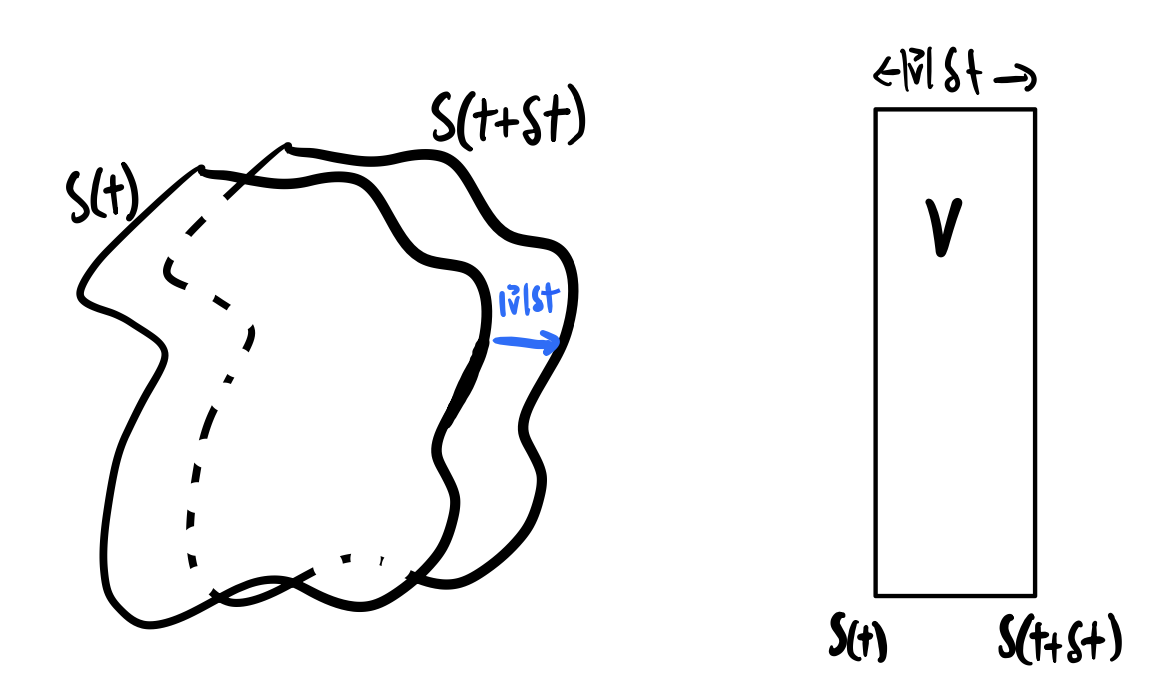
\includegraphics[scale=0.35]{Lectures/Images/lec16-twosurfacesinfini.png}
\end{center}

We consider the volume $V$ bounded by the surfaces + a ribbon of width $\abs{\v{v}}\delta t$. We notice that the magnetic flux over the entirety of its boundary (which is a closed surface) vanishes:
\begin{equation}
    \int_{\p V} \v{B} \cdot d\v{A} = 0
\end{equation}
which follows from Gauss' theorem and $\nabla \cdot \v{B} = 0$:
\begin{equation}
    0 = \int_{V}(0) dV =  \int_{V}(\nabla \cdot \v{B}) dV = \int_{\p V}\v{B} \cdot d\v{A}
\end{equation}
Thus, adding up the flux contributions from each face of the volume:
\begin{equation}
    0 = \int_{S(t + \delta t)}\v{B} \cdot d\v{A} - \int_{S(t)}\v{B} \cdot d\v{A} + \text{Ribbon contribution}
\end{equation}
Computing the contribution from the Ribbon element, we write the area element $d\v{A}$ in terms of a $d\v{l}$ line element:
\begin{equation}
    d\v{A} = d\v{l} \times \v{v}\delta t
\end{equation}
And thus the time derivative becomes:
\begin{equation}
    \frac{\delta}{\delta t}\int_{S(t)}\v{B} \cdot d\v{A} = -\int_{A \text{ ribbon}} \v{B} \cdot d\v{A} = -\int_{C(t)}\v{B} \cdot (d\v{l} \times \v{v})
\end{equation}
where $C(t)$ is the curve that goes around the Ribbon. 

\begin{center}
    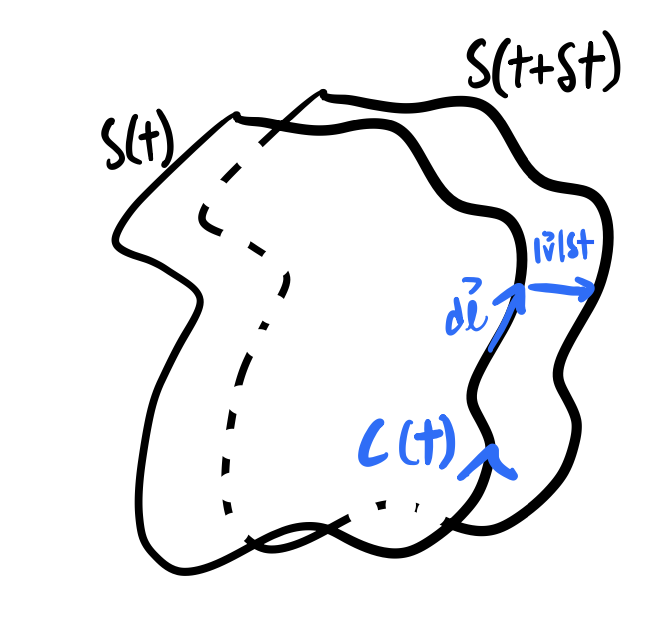
\includegraphics[scale=0.35]{Lectures/Images/lec16-circumference.png}
\end{center}

The $\delta t$ drops out because we divide by it when we take the derivative. Now:
\begin{equation}
    \frac{\delta}{\delta t}\int_{S(t)}\v{B} \cdot d\v{A} = -\int_{C(t)} (\v{v} \times \v{B}) \cdot d\v{l} \stackrel{\text{Stokes}}{=} -\int_{S(t)}(\nabla \times (\v{v} \times \v{B}))\cdot d\v{A}
\end{equation}
Thus, combining all terms:
\begin{equation}
     \dod{}{t}\int_{S(t)}\v{B} \cdot d\v{A} = \int d\v{A} \cdot (\dot{\v{B}} - \nabla \times (\v{v} \times \v{B})) = 0
\end{equation}
where the last equality follows from the induction equation.

\subsection{Wave solutions to the ideal MHD equations}
We had the five equations describing an ideal MHD fluid:
\begin{equation}
    \nabla \cdot \v{B} = 0
\end{equation}
\begin{equation}
    \dod{\rho_m}{t} + \nabla \cdot (\rho_m \v{v}) = 0
\end{equation}
\begin{equation}
    \rho_m\left(\dpd{}{t} + \v{v} \cdot \nabla\right)\v{v} = -\frac{1}{\mu_0}\v{B} \times (\nabla \times \v{B}) - \nabla p
\end{equation}
\begin{equation}
    \dot{\v{B}} = \nabla \times (\v{v} \times\v{B})
\end{equation}
\begin{equation}
    \dod{}{t}\left(\frac{p}{\rho^\gamma_M}\right) = \left(\dpd{}{t} + \v{v} \cdot \nabla\right)\left(\frac{p}{\rho^\gamma_m}\right) = 0
\end{equation}

We consider wavelike solutions to this fluid. We consider as our starting point to be the static solution:
\begin{equation}
    \v{B} = \v{B}_0
\end{equation}
\begin{equation}
    \v{v} = 0
\end{equation}
\begin{equation}
    \rho_M= \rho_{M0}
\end{equation}
\begin{equation}
    p = p_0
\end{equation}

On top of this we add the perturbations
\begin{equation}
    \v{B} = \v{B}_0 + \delta \v{B}(\v{x}, t)
\end{equation}
\begin{equation}
    \v{v} = \delta\v{v}(\v{x}, t)
\end{equation}
\begin{equation}
    \rho_M = \rho_{M0} + \delta \rho(\v{x}, t)
\end{equation}
Then to first order in the perturbations (discarding quadratic terms in the perturbation), the MHD equations become:
\begin{equation}
    \nabla \cdot \delta \v{B} = 0
\end{equation}
\begin{equation}
    \dpd{}{t}\delta \rho_{M} + \rho_{M0}\nabla \cdot \delta\v{v} = 0
\end{equation}
\begin{equation}
    \rho_{M0}\dpd{}{t}\delta \v{v} + \frac{1}{\mu_0}\v{B}_0 \times (\nabla \times \delta \v{B}) + \nabla \delta p = 0
\end{equation}
\begin{equation}
    -\dpd{}{t}\delta\v{B} + \nabla \times (\delta \v{v} \times \v{B}_0) = 0
\end{equation}

We look for wave solutions. There are three kinds of waves we can describe:
\begin{itemize}
    \item Suppose $\v{B}_0 = 0$. Then we just have a normal fluid, and get waves propagating with the speed $c_s = \dpd{p}{\rho}$.
    \item For $\v{B}_0 \neq 0$, we get magnetoacoustic waves (in some sense this is just a natural consequence of the normal fluid waves, by continuity). These waves have the property that $\nabla \cdot \delta \v{v} \neq 0$. This means that these waves are compressing the fluid, and they are longitudinal (c.f. electromagnetic waves which are transverse waves).
    \item Alfven waves. As an example, we take $\v{B}_0 = B_0\zhat$. Taking $\delta \rho_m = \delta p = 0$, $\delta \v{v} = \v{v}_1(t, z)$, $\delta \v{B} = \v{B}_1(t, z)$. We then must have that $\v{v}_1 \cdot \zhat = 0$, $\v{B}_1 \cdot \zhat = 0$. For these waves, we have $\nabla \cdot \delta \v{v} = 0$ (and of course $\nabla \cdot \delta \v{B} = 0$), which tells us the waves are not compression waves/the fluid is not compressed in this case. If we go through the math, what we find is the equations can be masssaged to the form:
    \begin{equation}
        \ddot{\v{v}}_1 - \frac{B_0^2}{\mu_0\rho_{M0}}\v{v}_1'' = 0
    \end{equation}
    which is a wave equation with the Alfven speed, describing Transverse waves:
    \begin{equation}
        c_A = \frac{B_0}{\sqrt{\mu_0 \rho_{M0}}}
    \end{equation}
\end{itemize}

\subsection{The Geometric Optics Approximation}
(Wald Ch.7) The last topic we will discuss is the connection between the description of light as an EM wave and as light rays.

Recall the wave equation:
\begin{equation}
    \square \psi = 0
\end{equation}
we've looked at $\psi = A_\mu, \v{E}, \v{B}$. When we talk about EM waves, we talk about solutions with frequency:
\begin{equation}
    \psi(t, \v{x}) = \chi(\v{x})e^{-i\omega t}
\end{equation}
If $\psi$ satisfies the wave equation, then $\chi$ satisfies the Helmholtz equation:
\begin{equation}
    \nabla^2 \chi + \frac{\omega^2}{c^2}\chi = 0
\end{equation}
The idea with geometrical optics are to look for solutions to this equation of the form:
\begin{equation}
    \chi(\v{x}) = A(\v{x})e^{iS(\v{x})}
\end{equation}
with $A(\v{x})$ the amplitude and $S(\v{x})$ the phase. In many settings (including light), one can find solutions to the Helmholtz equation that take this form.

Suppose we did the obvious thing and plugged in an ansatz of the above form. We would then find:
\begin{equation}
    (-\nabla S)^2 A + \nabla^2 A + \frac{\omega^2}{c^2}A + i(\nabla^2 S)A + 2i(\nabla S)\cdot(\nabla A) = 0
\end{equation}
The idea is to look for solutions of this equation where $S$ varies much more rapidly than $A$.

\begin{center}
    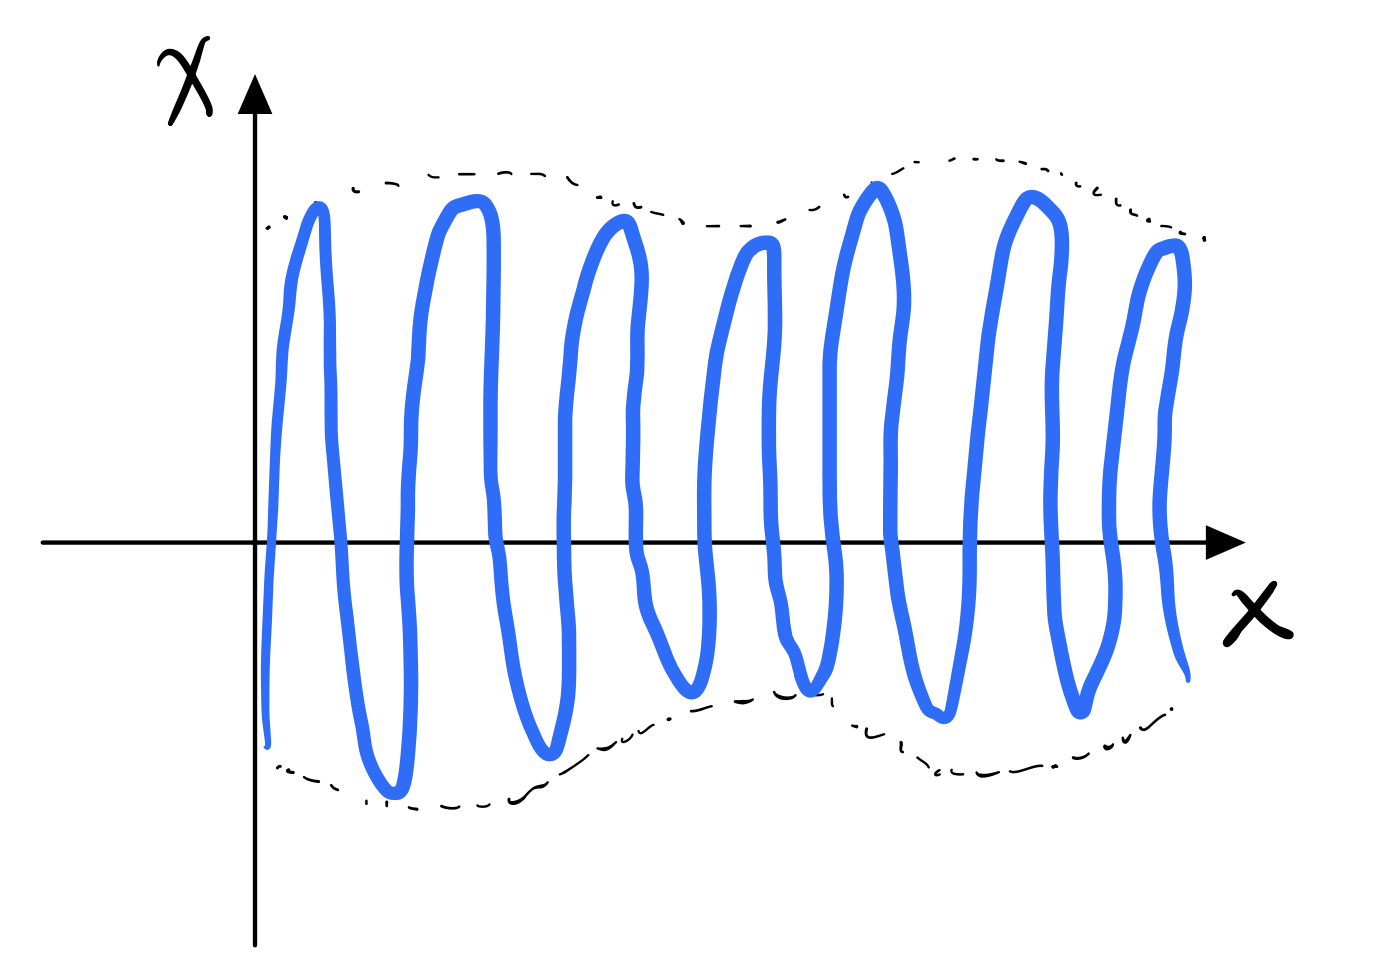
\includegraphics[scale=0.35]{Lectures/Images/lec16-phaseamp.png}
\end{center}

So, let's try to understand what happens under this assumption. If we want to assume:
\begin{equation}
    \frac{\abs{\nabla^2 A}}{A} \ll (\nabla S)^2
\end{equation}
This dimensionally says that:
\begin{equation}
    \frac{1}{L_A^2} \ll \frac{1}{L_S^2}
\end{equation}
Thus:
\begin{equation}
    L_S \ll L_A
\end{equation}
Thus we neglect the $\nabla^2 A$ term in the Helmholtz equation:\begin{equation}
    (-\nabla S)^2 A + \frac{\omega^2}{c^2}A + i(\nabla^2 S)A + 2i(\nabla S)\cdot(\nabla A) = 0
\end{equation}
The above equation then can be decomposed into a real and imaginary equation that must individually be satisfied:
\begin{equation}
    (\nabla S)^2 = \frac{\omega^2}{c^2}
\end{equation}
\begin{equation}
    2\nabla S \cdot \nabla A + (\nabla^2 S)A = 0
\end{equation}
Which is known as the geometric optics approximation, or also known as the WKB approximation.

Thus, if we define:
\begin{equation}
    \v{k} = \nabla S
\end{equation}
then the real part of the equation looks like:
\begin{equation}
    \abs{\v{k}}^2 = \frac{\omega^2}{c^2}
\end{equation}
This looks like what we have seen before when we looked at EM waves, but there is an important distinction - there, $\v{k}$ was a fixed vector in the ansatz. Here, $\v{k}$ is not fixed, but rather $\v{k}$, like $S$, may depend on $\v{x}$.